\documentclass[conference]{IEEEtran}
\usepackage{cite}
\usepackage{amsmath,amssymb,amsfonts}
\usepackage{algorithmic}
\usepackage{graphicx}
\usepackage{textcomp}
\usepackage{xcolor}
\usepackage{listings}
\usepackage{hyperref}
\usepackage{tikz}
\usepackage{pgfplots}
\pgfplotsset{compat=1.17}
\usetikzlibrary{shapes,arrows,positioning,calc}

% Define a soft background color for the code blocks
\definecolor{codebg}{RGB}{245,245,248}

% Code listing style configuration
\lstset{
  language=C++,
  backgroundcolor=\color{codebg}, 
  basicstyle=\ttfamily\scriptsize, 
  keywordstyle=\color{blue},
  commentstyle=\color{green!60!black},
  stringstyle=\color{purple},
  breaklines=true,
  showstringspaces=false,
  frame=single,
  rulecolor=\color{gray!50}, 
  xleftmargin=0.5em,  
  xrightmargin=0.5em, 
  captionpos=b
}

\begin{document}

\title{Adaptive Optical Telemetry: Evolving from Visible Light Baselines to Infrared Stepwise Derivative Thresholding}

\author{Kartik Lahoti, Puni Aditya \\
\textit{Department of Electrical Engineering} \\
\textit{IIT Hyderabad}
}

\maketitle

\begin{abstract}
Optical wireless communication offers a license-free alternative to Radio Frequency (RF) systems. However, simple visible light links utilizing Light Dependent Resistors (LDRs) face significant challenges regarding ambient light interference and hardware latency. This paper outlines a comprehensive two-stage development of a Morse Code On-Off Keying (OOK) system. Phase I establishes a baseline Visible Light Communication (VLC) link, documenting a maximum range of 27 cm and identifying the ``Iceberg Effect'' of signal truncation. Phase II introduces a novel technological evolution: the transition to the Infrared (IR) spectrum coupled with a Stepwise Derivative Method (SDM) for adaptive thresholding. By utilizing software-based dynamic noise-floor tracking and optimizing hardware impedance from 10k$\Omega$ to 1M$\Omega$, the system overcomes environmental DC bias, successfully extending the effective transmission range by over 581\% to 1.57 meters while maintaining 100\% decoding accuracy on a 7-segment hardware interface.
\end{abstract}

\begin{IEEEkeywords}
Visible Light Communication (VLC), Infrared (IR), Stepwise Derivative Method (SDM), On-Off Keying (OOK), Morse Code, Adaptive Thresholding.
\end{IEEEkeywords}

\section{Introduction}
Wireless optical communication is highly dependent on clear Line-of-Sight (LoS) and a high Signal-to-Noise Ratio (SNR). In entry-level embedded systems, a standard Light Emitting Diode (LED) paired with a Light Dependent Resistor (LDR) is commonly used to demonstrate data transfer. However, ambient environmental lighting introduces a severe DC bias into the receiver, and LDRs exhibit significant photo-conductive latency.

The novelty of this paper lies in its evolutionary approach to solving these physical layer limitations. We first establish a baseline VLC system to document the hardware-induced signal degradation known as the ``Iceberg Effect.'' Following this, we introduce an advanced Infrared (IR) iteration. The core innovation of this second phase is the Stepwise Derivative Method (SDM), a software-defined signal processing algorithm that calculates a rolling average of the ambient noise floor to establish a dynamic, self-calibrating threshold. This transition from static visible light sensing to adaptive IR telemetry, combined with trans-impedance optimization at the receiver, represents a significant leap in communication reliability.

\subsection{Related Works and Novelty}
Standard commercial IR systems avoid ambient noise by utilizing 38kHz Carrier Waves and specialized TSOP receiver modules. While effective, these modules act as ``black boxes'' that strip the analog signal data away from the microcontroller, preventing custom low-level signal analysis. Conversely, standard unmodulated photodiode circuits use fixed analog thresholds that fail the moment room lighting changes. Our proposed SDM bridges this gap: it retains the raw analog data of a simple photodiode circuit but applies a dynamic digital moving-average filter to reject ambient DC bias. This ``cross-layer'' approach allows for unparalleled customizability in low-cost hardware.

\subsection{Baud Rate and Telemetry Applicability}
Morse code, utilizing OOK, possesses a fundamentally low baud rate compared to modern digital modulation schemes like UART or QAM. However, for specialized telemetry applications—such as underwater optical communication, emergency beacons, or low-cost sensor nodes—signal penetration and robustness take precedence over raw speed. The widened tolerance windows used in this paper's decoding logic demonstrate how low baud rate systems can reliably reconstruct highly degraded signals where high-speed protocols would experience catastrophic packet loss.

\begin{figure}[htbp]
    \centering
    \resizebox{\columnwidth}{!}{
    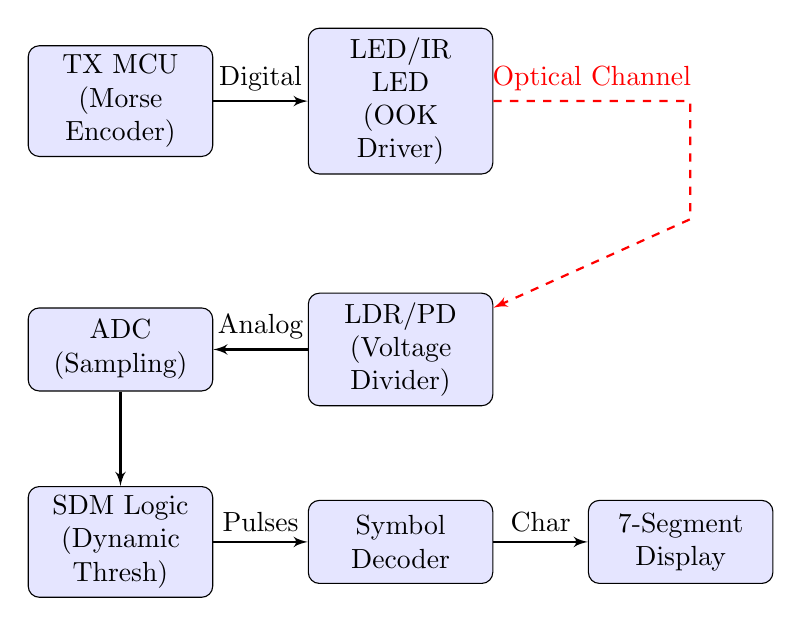
\begin{tikzpicture}[node distance=1.2cm, auto, >=stealth]
        \tikzstyle{block} = [rectangle, draw, fill=blue!10, text width=6em, text centered, rounded corners, minimum height=3em]
        \tikzstyle{line} = [draw, -latex', thick]
        
        % TX Nodes
        \node [block] (mcu1) {TX MCU\\(Morse Encoder)};
        \node [block, right=of mcu1] (led) {LED/IR LED\\(OOK Driver)};
        
        % Channel
        % CHANGED: Increased right distance from 1cm to 2.5cm to prevent text overlap
        \node [coordinate, right=2.5cm of led] (ch1) {}; 
        \node [coordinate, below=1.5cm of ch1] (ch2) {};
        
        % RX Nodes
        \node [block, below=1.5cm of led] (sensor) {LDR/PD\\(Voltage Divider)};
        \node [block, left=of sensor] (adc) {ADC\\(Sampling)};
        \node [block, below=of adc] (sdm) {SDM Logic\\(Dynamic Thresh)};
        \node [block, right=of sdm] (decoder) {Symbol\\Decoder};
        \node [block, right=of decoder] (disp) {7-Segment\\Display};

        % Paths
        \path [line] (mcu1) -- node {Digital} (led);
        \path [line, dashed, red] (led) -- node[above] {Optical Channel} (ch1) -- (ch2) -- (sensor);
        \path [line] (sensor) -- node[above] {Analog} (adc);
        \path [line] (adc) -- (sdm);
        \path [line] (sdm) -- node[above] {Pulses} (decoder);
        \path [line] (decoder) -- node[above] {Char} (disp);
    \end{tikzpicture}
    }
    \caption{System Block Diagram detailing the cross-layer flow from hardware transmission to the software-defined SDM filtering and hardware output.}
    \label{fig:block}
\end{figure}
\section{Phase I: Visible Light Baseline}

\subsection{Circuit Implementation}
The baseline system operates entirely in the visible spectrum. 
\begin{itemize}
    \item \textbf{Transmitter (TX):} An Arduino microcontroller drives a standard visible LED. The LED's anode connects to Digital Pin 5, while the cathode grounds through a $220\Omega$ current-limiting resistor. 
    \item \textbf{Receiver (RX):} The optical sensor is a Light Dependent Resistor (LDR) arranged in a voltage divider. The 5V supply is connected to one leg of the LDR. The secondary leg connects to the Arduino's Analog Pin A0 and a $10\text{k}\Omega$ pull-down resistor connected to ground. 
\end{itemize}

\subsection{Hardware Latency and The ``Iceberg Effect''}
When bridging analog optical sensing and digital microcontrollers, signal truncation occurs. As shown in Fig. \ref{fig:iceberg}, an expected ``Dah'' signal transmitted for 600ms is detected for a fraction of that time. LDRs exhibit notable rise/fall latency, resulting in a trapezoidal curve rather than a square wave. To counteract this, our receiver employs widened tolerance windows (e.g., 400ms to 900ms).

\begin{figure}[htbp]
    \centering
    \resizebox{\columnwidth}{!}{
    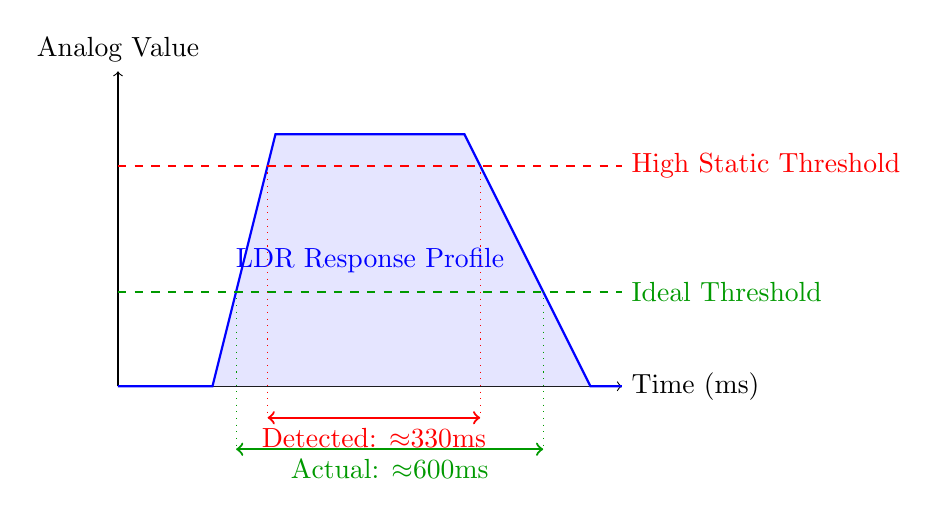
\begin{tikzpicture}[scale=0.8]
        \draw[->] (0,0) -- (8,0) node[right] {Time (ms)};
        \draw[->] (0,0) -- (0,5) node[above] {Analog Value};
        \draw[thick, blue, fill=blue!10] (0,0) -- (1.5,0) -- (2.5,4) -- (5.5,4) -- (7.5,0) -- (8,0);
        \node[blue] at (4, 2) {LDR Response Profile};
        \draw[red, thick, dashed] (0,3.5) -- (8,3.5);
        \node[red, right] at (8,3.5) {High Static Threshold};
        \draw[green!60!black, thick, dashed] (0,1.5) -- (8,1.5);
        \node[green!60!black, right] at (8,1.5) {Ideal Threshold};
        \draw[dotted, red] (2.375, 3.5) -- (2.375, -0.5); 
        \draw[dotted, red] (5.75, 3.5) -- (5.75, -0.5); 
        \draw[dotted, green!60!black] (1.875, 1.5) -- (1.875, -1);   
        \draw[dotted, green!60!black] (6.75, 1.5) -- (6.75, -1);   
        \draw[<->, red, thick] (2.375, -0.5) -- (5.75, -0.5) node[midway, below] {Detected: $\approx$330ms};
        \draw[<->, green!60!black, thick] (1.875, -1) -- (6.75, -1) node[midway, below] {Actual: $\approx$600ms};
    \end{tikzpicture}
    }
    \caption{The ``Iceberg Effect'' illustrating temporal truncation caused by improper static thresholding of an LDR signal.}
    \label{fig:iceberg}
\end{figure}

\subsection{Visible Light Results}
The baseline system achieved a maximum reliable transmission distance of only 11-12 cm in room light, and 27 cm in total darkness. These results highlight the environmental fragility of unmodulated VLC.

\section{Phase II: Infrared Evolution and SDM}

\subsection{Circuit Implementation}
To resolve the noise and range issues of Phase I, the physical layer was upgraded to a 940nm Infrared (IR) ecosystem.
\begin{itemize}
    \item \textbf{Transmitter (TX):} The visible LED is replaced by an IR LED. The anode (long leg) connects to Digital Pin 5, and the cathode connects to ground via a $220\Omega$ resistor.
    \item \textbf{Receiver (RX) Sensor:} A high-speed IR photodiode replaces the LDR, operating in reverse-bias mode. The cathode (short leg) connects to 5V. The anode (long leg) connects to Analog Pin A0 and a pull-down load resistor ($R_L$) to ground.
    \item \textbf{Receiver (RX) Display:} A Common Anode 7-segment display provides real-time character output. The common pin connects to 5V, while segments A through G connect to Digital Pins 2 through 8 via $220\Omega$ current-limiting resistors.
\end{itemize}

\subsection{Hardware Optimization: Trans-Impedance Gain}
Because a photodiode in reverse-bias produces a photocurrent ($I_{pd}$) proportional to the incident photon flux, the voltage sampled by the ADC is governed by Ohm's Law: $V_{adc} = I_{pd} \times R_L$, where $R_L$ is the pull-down load resistor.
\begin{itemize}
    \item With a standard **$10\text{k}\Omega$ resistor**, the voltage swing was insufficient for weak signals at a distance, limiting the range to **47 cm**.
    \item By increasing to a **$1\text{M}\Omega$ resistor**, sensitivity was maximized. The high impedance amplified the minute photocurrents generated by distant IR pulses, extending the raw range to **1.57 meters**.
\end{itemize}

\subsection{Stepwise Derivative Method (SDM)}
While the $1\text{M}\Omega$ hardware configuration provides immense gain, it simultaneously amplifies ambient environmental noise (e.g., thermal fluctuations and background IR). To isolate the transmission pulses, we developed the Stepwise Derivative Method (SDM). 

The algorithm maintains a rolling buffer of $N=10$ discrete analog readings to calculate a floating real-time average ($V_{noise}$) of the ambient environment. The equations governing the SDM are as follows:

\begin{align}
    V_{noise}[n] &= \frac{1}{N} \sum_{i=0}^{N-1} V_{adc}[n-i] \label{eq:noise} \\
    V_{threshold}[n] &= V_{noise}[n] + \sigma \label{eq:thresh}
\end{align}

Where $\sigma$ represents the `signalMargin`, a defined constant (set to 30) that ensures only intentional high-intensity peaks surpass the moving baseline. 

\textbf{Note on Resistance Variation:} When varying the trans-impedance resistor $R_L$ from 10k$\Omega$ to 1M$\Omega$ to increase range, the baseline thermal noise also scales. Consequently, the $\sigma$ (`signalMargin`) variable in the SDM code must be empirically adjusted (e.g., raised from 30 to 45) to prevent false triggering from amplified background flicker.

\section{Experimental Results and Conclusion}
The integration of impedance-tuned hardware and SDM software yielded profound improvements. As illustrated in Fig. \ref{fig:graph}, the visible light baseline failed abruptly at 27 cm. The unoptimized IR setup ($10\text{k}\Omega$) reached 47 cm. However, the fully optimized IR-SDM setup ($1\text{M}\Omega$) successfully maintained 100\% decoding accuracy up to 157 cm.

\begin{figure}[htbp]
    \centering
    \resizebox{0.9\columnwidth}{!}{
    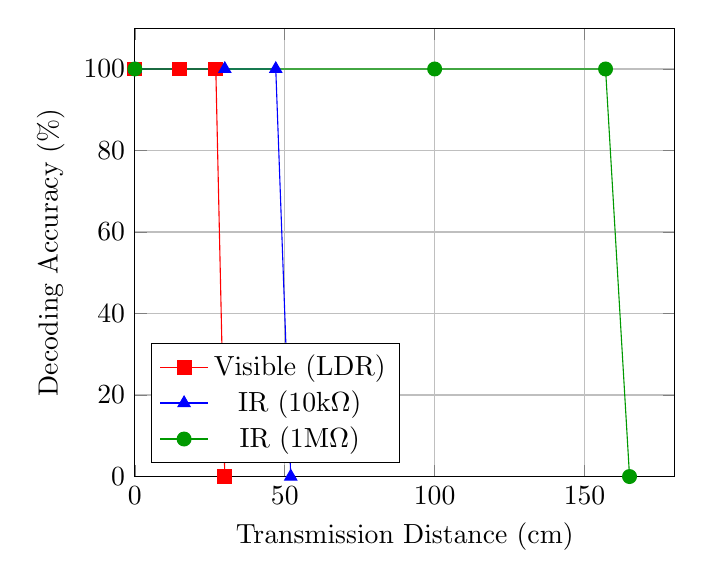
\begin{tikzpicture}
        \begin{axis}[
            xlabel={Transmission Distance (cm)},
            ylabel={Decoding Accuracy (\%)},
            xmin=0, xmax=180,
            ymin=0, ymax=110,
            legend pos=south west,
            grid=both,
            mark size=2.5pt
        ]
        \addplot[color=red, mark=square*] coordinates {(0,100) (15,100) (27,100) (30,0)}; 
        \addplot[color=blue, mark=triangle*] coordinates {(0,100) (30,100) (47,100) (52,0)}; 
        \addplot[color=green!60!black, mark=*] coordinates {(0,100) (100,100) (157,100) (165,0)}; 
        \legend{Visible (LDR), IR ($10\text{k}\Omega$), IR ($1\text{M}\Omega$)}
        \end{axis}
    \end{tikzpicture}
    }
    \caption{Comparative analysis of decoding accuracy over distance across the three hardware configurations.}
    \label{fig:graph}
\end{figure}

This research demonstrates that reliable, long-range optical telemetry does not explicitly require complex frequency modulation hardware. By employing a cross-layer design—maximizing analog gain via high-impedance loads while utilizing digital SDM equations to reject the resultant DC bias—a simple OOK embedded system can achieve robust telemetry across varying environments.

% \appendices
% \section{Phase I: Visible Light Source Code}
% \begin{lstlisting}[caption={Visible Light TX Code}]
% const int ledPin = 5;
% const int ditTime = 200;
% const int dahTime = 600;
% const int symbolGap = 200;
% const int letterGap = 600;
% const int wordGap = 1400;

% String letters[] = {
  % ".-", "-...", "-.-.", "-..", ".", "..-.", "--.", "....", "..", 
  % ".---", "-.-", ".-..", "--", "-.", "---", ".--.", "--.-", ".-.", 
  % "...", "-", "..-", "...-", ".--", "-..-", "-.--", "--.." 
% };

% void setup() { pinMode(ledPin, OUTPUT); }

% void flash(int duration) {
  % digitalWrite(ledPin, HIGH);
  % delay(duration);
  % digitalWrite(ledPin, LOW);
  % delay(symbolGap);
% }

% void sendChar(char c) {
  % if (c >= 'A' && c <= 'Z') {
    % String morse = letters[c - 'A'];
    % for (int i = 0; i < morse.length(); i++) {
      % if (morse[i] == '.') flash(ditTime);
      % else if (morse[i] == '-') flash(dahTime);
    % }
    % delay(letterGap - symbolGap); 
  % } 
  % else if (c == ' ') { delay(wordGap - symbolGap); }
% }

% void loop() {
  % String input = "HELLO WORLD";
  % input.toUpperCase();
  % for (int i = 0; i < input.length(); i++) { sendChar(input[i]); }
  % delay(5000);
% }
% \end{lstlisting}

% \begin{lstlisting}[caption={Visible Light RX Code}]
% const int ldrPin = A0;
% const int threshold = 90;
% unsigned long startTime = 0;
% unsigned long darkStartTime = 0;
% bool isLight = false;
% String currentLetter = "";

% void loop() {
  % int sensorValue = analogRead(ldrPin);
  % if (sensorValue > threshold) {
    % if (!isLight) { startTime = millis(); isLight = true; }
    % darkStartTime = millis(); 
  % } else {
    % if (isLight) {
      % unsigned long duration = millis() - startTime;
      % if (duration >= 100 && duration <= 350) currentLetter += ".";
      % else if (duration >= 400 && duration <= 800) currentLetter += "-";
      % isLight = false;
      % darkStartTime = millis();
    % } else {
      % unsigned long darkDuration = millis() - darkStartTime;
      % if (darkDuration > 500 && currentLetter != "") {
        % Serial.print(decodeMorse(currentLetter));
        % currentLetter = "";
      % }
    % }
  % }
% }
% \end{lstlisting}

% \section{Phase II: Infrared SDM Implementation}
% \begin{lstlisting}[caption={Infrared Transmitter (TX) Code}]
% const int irLedPin = 5; 
% const int ditTime = 200;
% const int dahTime = 600;
% const int symbolGap = 200;
% const int letterGap = 800;
% const int wordGap = 2000;

% void setup() { 
  % pinMode(irLedPin, OUTPUT); 
  % Serial.begin(9600);
  % Serial.println("Transmitter Ready.");
% }

% void flash(int duration) {
  % digitalWrite(irLedPin, HIGH);
  % delay(duration);
  % digitalWrite(irLedPin, LOW);
  % delay(symbolGap);
% }

% void sendMorse(char c) {
  % c = toupper(c);
  % switch (c) {
    % case 'A': flash(ditTime); flash(dahTime); break;
    % case 'B': flash(dahTime); flash(ditTime); flash(ditTime); flash(ditTime); break;
    % case 'C': flash(dahTime); flash(ditTime); flash(dahTime); flash(ditTime); break;
    % case 'D': flash(dahTime); flash(ditTime); flash(ditTime); break;
    % case 'E': flash(ditTime); break;
    % case 'F': flash(ditTime); flash(ditTime); flash(dahTime); flash(ditTime); break;
    % case 'G': flash(dahTime); flash(dahTime); flash(ditTime); break;
    % case 'H': flash(ditTime); flash(ditTime); flash(ditTime); flash(ditTime); break;
    % case 'I': flash(ditTime); flash(ditTime); break;
    % case 'J': flash(ditTime); flash(dahTime); flash(dahTime); flash(dahTime); break;
    % case 'K': flash(dahTime); flash(ditTime); flash(dahTime); break;
    % case 'L': flash(ditTime); flash(dahTime); flash(ditTime); flash(ditTime); break;
    % case 'M': flash(dahTime); flash(dahTime); break;
    % case 'N': flash(dahTime); flash(ditTime); break;
    % case 'O': flash(dahTime); flash(dahTime); flash(dahTime); break;
    % case 'P': flash(ditTime); flash(dahTime); flash(dahTime); flash(ditTime); break;
    % case 'Q': flash(dahTime); flash(dahTime); flash(ditTime); flash(dahTime); break;
    % case 'R': flash(ditTime); flash(dahTime); flash(ditTime); break;
    % case 'S': flash(ditTime); flash(ditTime); flash(ditTime); break;
    % case 'T': flash(dahTime); break;
    % case 'U': flash(ditTime); flash(ditTime); flash(dahTime); break;
    % case 'V': flash(ditTime); flash(ditTime); flash(ditTime); flash(dahTime); break;
    % case 'W': flash(ditTime); flash(dahTime); flash(dahTime); break;
    % case 'X': flash(dahTime); flash(ditTime); flash(ditTime); flash(dahTime); break;
    % case 'Y': flash(dahTime); flash(ditTime); flash(dahTime); flash(dahTime); break;
    % case 'Z': flash(dahTime); flash(dahTime); flash(ditTime); flash(ditTime); break;
    % case ' ': delay(wordGap - symbolGap); break;
  % }
  % delay(letterGap - symbolGap);
% }

% void loop() {
  % String input = "HELLO WORLD";
  % input.trim();
  % for (int i = 0; i < input.length(); i++) { sendMorse(input[i]); }
  % delay(15000UL);
% }
% \end{lstlisting}

% \begin{lstlisting}[caption={Infrared Receiver (RX) Code: SDM Algorithm \& 10k$\Omega$ Base}]
% // --- IR Receiver (RX): SDM + Morse + 7-Segment ---
% const int irPin = A0;

% const int numReadings = 10;
% int readings[numReadings];      
% int readIndex = 0;              
% long total = 0;                  
% int averageNoise = 0;                
% const int signalMargin = 30; // 10kOhm baseline margin
% int dynamicThreshold = 0;

% unsigned long startTime = 0;
% unsigned long darkStartTime = 0;
% bool isLight = false;
% bool spaceSent = true; 
% String currentLetter = "";

% String morseDict[] = {
  % ".-", "-...", "-.-.", "-..", ".", "..-.", "--.", "....", "..",
  % ".---", "-.-", ".-..", "--", "-.", "---", ".--.", "--.-", ".-.",
  % "...", "-", "..-", "...-", ".--", "-..-", "-.--", "--.."
% };

% const int segPins[7] = {2, 3, 4, 5, 6, 7, 8};

% // Common Anode Logic (0=ON, 1=OFF)
% const byte font[26][7] = {
  % {0,0,0,1,0,0,0}, {1,1,0,0,0,0,0}, {0,1,1,0,0,0,1}, {1,0,0,0,0,1,0}, 
  % {0,1,1,0,0,0,0}, {0,1,1,1,0,0,0}, {0,1,0,0,0,0,0}, {1,0,0,1,0,0,0}, 
  % {1,1,1,1,0,0,1}, {1,0,0,0,1,1,1}, {1,0,1,0,0,0,0}, {1,1,1,0,0,0,1}, 
  % {0,0,1,0,1,0,0}, {1,1,0,1,0,1,0}, {0,0,0,0,0,0,1}, {0,0,1,1,0,0,0}, 
  % {0,0,0,1,1,0,0}, {1,1,1,1,0,1,0}, {0,1,0,0,1,0,0}, {1,1,1,0,0,0,0}, 
  % {1,0,0,0,0,0,1}, {1,0,0,0,0,0,1}, {1,0,1,0,0,0,1}, {1,0,0,1,0,0,0}, 
  % {1,0,0,0,1,0,0}, {0,0,1,0,0,1,0}
% };

% void setup() {
  % Serial.begin(9600);
  % for (int i = 0; i < 7; i++) {
    % pinMode(segPins[i], OUTPUT);
    % digitalWrite(segPins[i], HIGH);
  % }
  % for (int i = 0; i < numReadings; i++) readings[i] = 0;
  % Serial.println("System Active...");
% }

% char decodeMorse(String morse) {
  % for (int i = 0; i < 26; i++) {
    % if (morseDict[i] == morse) return (char)('A' + i);
  % }
  % return '?'; 
% }

% void displayChar(char c) {
  % if (c >= 'A' && c <= 'Z') {
    % int index = c - 'A';
    % for (int i = 0; i < 7; i++) digitalWrite(segPins[i], font[index][i]);
  % } else {
    % for (int i = 0; i < 7; i++) digitalWrite(segPins[i], HIGH); 
  % }
% }

% void loop() {
  % int sensorValue = analogRead(irPin);

  % // 1. SDM Algorithm
  % total = total - readings[readIndex];
  % readings[readIndex] = sensorValue;
  % total = total + readings[readIndex];
  % readIndex = (readIndex + 1) % numReadings;
  % averageNoise = total / numReadings;
  % dynamicThreshold = averageNoise + signalMargin;

  % // 2. Pulse Edge Detection
  % if (sensorValue > dynamicThreshold) {
    % if (!isLight) { startTime = millis(); isLight = true; }
    % darkStartTime = millis(); 
    % spaceSent = false;
  % } else {
    % if (isLight) {
      % unsigned long duration = millis() - startTime;
      % if (duration >= 100 && duration <= 350) { currentLetter += "."; Serial.print("."); }
      % else if (duration >= 400 && duration <= 800) { currentLetter += "-"; Serial.print("-"); }
      % isLight = false;
      % darkStartTime = millis();
    % } else {
      % unsigned long darkDuration = millis() - darkStartTime;
      
      % // End of Letter Logic
      % if (darkDuration > 600 && currentLetter != "") {
        % char decoded = decodeMorse(currentLetter);
        % Serial.print(" ["); Serial.print(decoded); Serial.print("] ");
        % displayChar(decoded); 
        % delay(1200); 
        % displayChar(' '); 
        % currentLetter = "";   
        
        % // SDM Fast-Forward Reset
        % int currentLight = analogRead(irPin);
        % for(int i=0; i<numReadings; i++) readings[i] = currentLight;
        % total = currentLight * numReadings;
      % }
      
      % // Space (Word Gap) Logic
      % if (darkDuration > 3000 && !spaceSent) {
        % Serial.print("   "); 
        % spaceSent = true;
      % }
    % }
  % }
% }
% \end{lstlisting}

\end{document}